\documentclass[aspectratio=169]{beamer}
\usetheme{metropolis} % Choose a professional theme
\usepackage{graphicx} % Required package for including images
\usepackage{enumitem} % Required package for customizing itemize environment
\usepackage{listings}
\usepackage{colortbl}

\title{Localization of Neural Sources from Simulated EEG Data}
\author{Kamilla Ida Julie Sulebakk}
\date{\today}

\begin{document}
\maketitle

\begin{frame}{Agenda}
    \begin{itemize}
        \item[$\bullet$] Background -- the EEG inverse problem and its relevance for medical diagnosis
        \item[$\bullet$] NY Head Model and the generation of EEG signals
        \item[$\bullet$] Basic neural network architectures
        \item[$\bullet$] Results and analysis
        \item[$\bullet$] Personal takeaways
    \end{itemize}
\end{frame}





\begin{frame}{Background}
    \begin{itemize}
        \item[$\bullet$] EEG inverse problem
        \begin{itemize}
            \item[\tiny$\blacksquare$] Localize the neural populations that are generating specific EEG signal components
        \end{itemize}
        \item[$\bullet$] Seizure zone in EEG recordings from patients with epilepsy
        \item[$\bullet$] Neural networks for the purpose of localizing abnormal activity, can serve as a supplement for analysis

    \end{itemize}
\end{frame}





\begin{frame}{Simulating EEG Data}
    \begin{columns}
        \begin{column}{0.5\textwidth}
            \begin{itemize}[leftmargin=1em,labelindent=\dimexpr1em-\labelsep]
                \item[$\bullet$] \footnotesize Substantial amount of data is necessary to:
                \begin{itemize}
                    \item[\tiny$\blacksquare$] \scriptsize Capture complicated relationships
                    \item[\tiny$\blacksquare$] \scriptsize Make accurate predictions
                    \item[\tiny$\blacksquare$] \scriptsize Generalize well to unseen examples
                \end{itemize}
                \item[$\bullet$] \footnotesize True EEG data for training a NN doesn't exist
                \item[$\bullet$] \footnotesize Solution: Simulate realistic data using LFPy
                \item[$\bullet$] \footnotesize New York Head Model
                \begin{itemize}
                    \item[\tiny$\blacksquare$] \scriptsize Volume conductor, computer model of the human head
                    \item[\tiny$\blacksquare$] \scriptsize Simulates electrical activity in the brain
                    \item[\tiny$\blacksquare$] \scriptsize Based on the anatomical and electrical characteristicsof MRI data
                    \item[\tiny$\blacksquare$] \scriptsize Provides detailed information on geometry and electrical properties
                    \item[\tiny$\blacksquare$] \scriptsize Generates predictions of EEG signals at 231 electrodes for 75K cortical locations
                    \item[\tiny$\blacksquare$] \scriptsize Utilizes the "Lead Field Matrix"
                \end{itemize}
            \end{itemize}
        \end{column}
        \begin{column}{0.5\textwidth}
            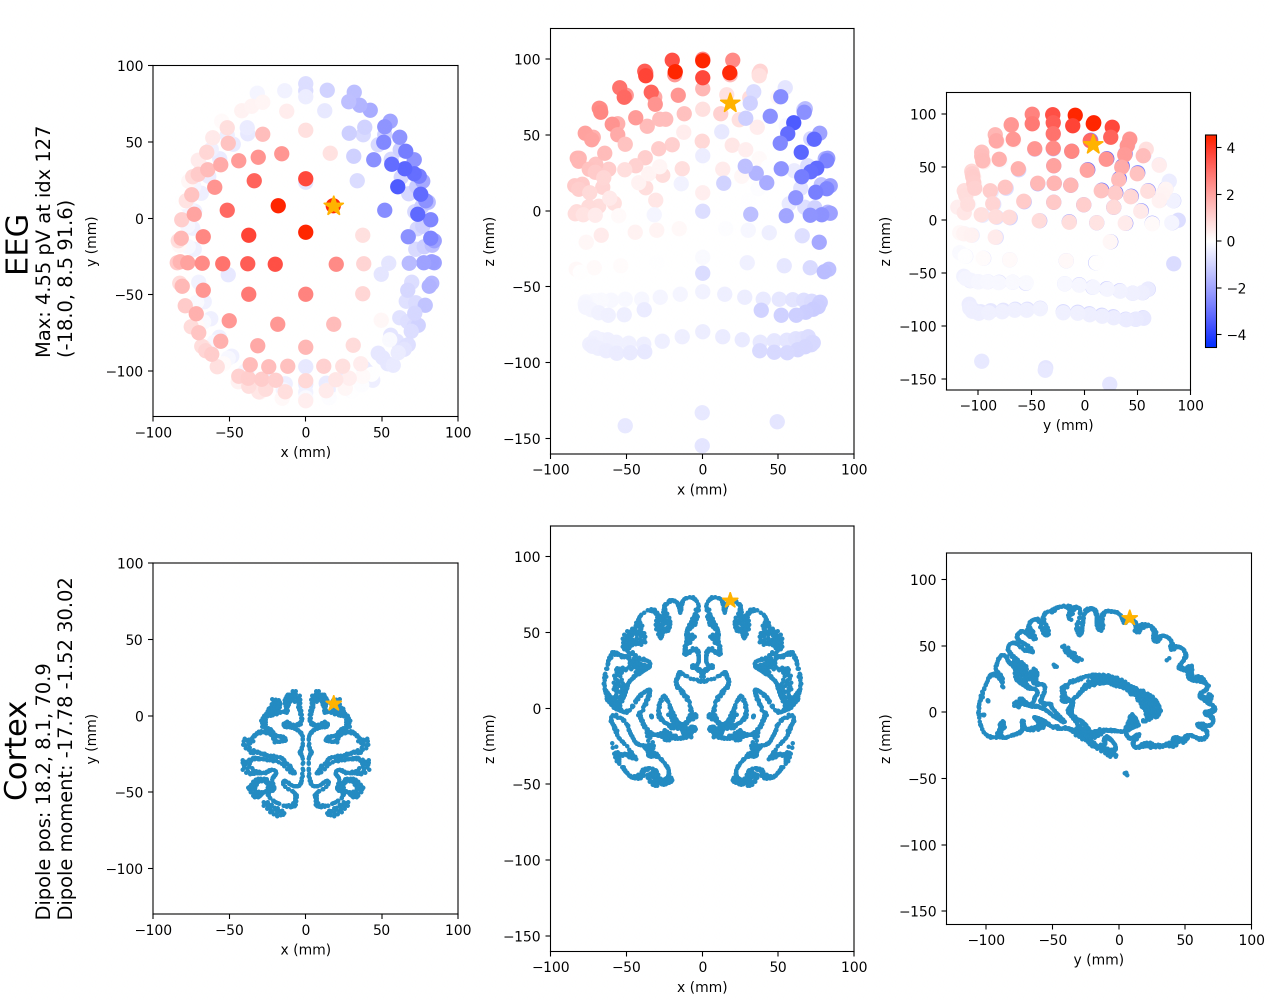
\includegraphics[width=\textwidth]{figures/cortex.png}
        \end{column}
    \end{columns}
\end{frame}


\begin{frame}{Current Dipole Approximation}
    \begin{columns}
        \begin{column}{0.5\textwidth}
            \begin{itemize}
              \item[$\bullet$] When simulating EEG signals, neural sources are treated as current dipoles
              \item[$\bullet$] Electrical potentials stemming from neural activity of a population of neurons tend to look like current dipoles
              \item[$\bullet$] By doing a multipole expansion the extracellular potential can be approximated by the dipole contribution alone
            \end{itemize}
        \end{column}
        \begin{column}{0.5\textwidth}
            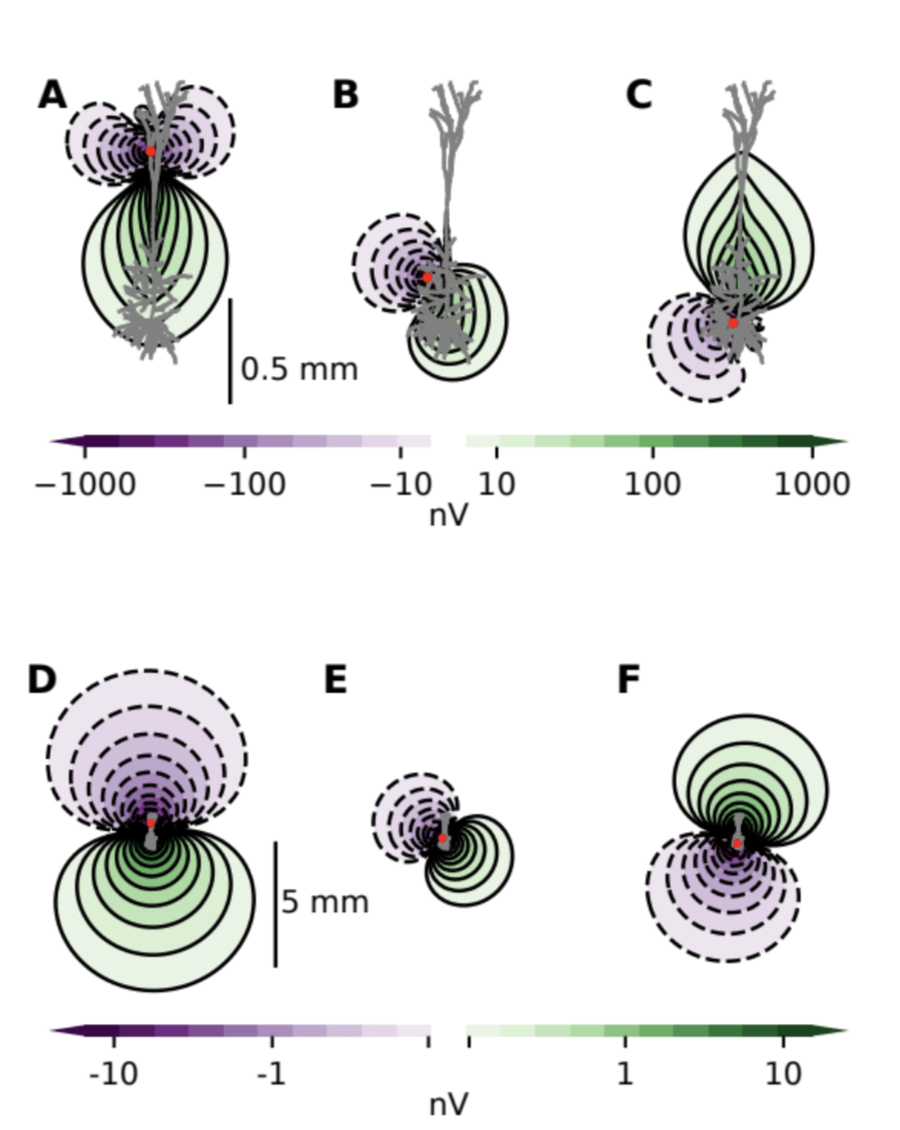
\includegraphics[width=0.7\textwidth]{figures/dipole_pattern.png}
        \end{column}
    \end{columns}
\end{frame}



\begin{frame}[fragile]{Code snippet}
\begin{lstlisting}[language=Python, frame=single, basicstyle=\fontsize{6}{6}\selectfont]
def calculate_eeg(nyhead: NYHeadModel, A: int = 1.0):
    """
    Calculates the eeg signal from the dipole population

    returns:
        eeg_i : array of length (231)
            Combined eeg signal from the dipole population for a single patient
    """
    M = nyhead.get_transformation_matrix()

    # Dipole oriented in depth direction in the cortex
    p = np.array(([0.0], [0.0], [A])) * 1E7 # [nA* mu m]

    # Rotates the direction of the dipole moment so that it is normal to the cerebral cortex
    p = nyhead.rotate_dipole_to_surface_normal(p)

    # Generates the EEG signal that belongs to the dipole moment
    eeg_i = M @ p * 1E3 # [mV] -> muV unit conversion (eeg_i between 10 og 100)

    return eeg_i
\end{lstlisting}
\end{frame}





% \begin{frame}[fragile]{Code snippet (2)}
% \begin{lstlisting}[language=Python, frame=single, basicstyle=\fontsize{6}{6}\selectfont]
% def return_simple_dipole(num_samples:int, num_dipoles: int = 1):
%     """
%     Produce eeg data from single dipole moment for num_samples
%
%     input:
%         num_samples : int
%             The number of samples/patients
%
%         num_dipoles : int
%             The number of desired diples
%
%     returns:
%         eeg : numpy array of floats, size (num_samples, 231)
%             Electrical signals from single dipole in the cortex
%
%         dipole_locations : numpy array of floats, size (3, num_samples)
%             Position of single dipole for each sample
%     """
%     nyhead = NYHeadModel()
%
%     rng = np.random.default_rng(seed=36)
%     dipole_locations = rng.choice(nyhead.cortex, size=num_samples, axis=1) # [mm]
%
%     eeg = np.zeros((num_samples, 231))
%
%     for i in range(num_samples):
%         nyhead.set_dipole_pos(dipole_locations[:,i])
%         eeg_i = calculate_eeg(nyhead)
%         eeg[i, :] = eeg_i.T
%
%     return eeg, dipole_locations
% \end{lstlisting}
% \end{frame}





\begin{frame}{The Feed Forward Neural Network}
    \begin{columns}
        \begin{column}{0.5\textwidth}
            \begin{itemize}
                \item[$\bullet$] "Learns from experience"
                \begin{itemize}
                    \item[\tiny$\blacksquare$] Processing and analyzing data
                    \item[\tiny$\blacksquare$] Uncover patterns linking input features to their corresponding output values
                \end{itemize}
                \item[$\bullet$] FFNN: Information is only processed forward
                \begin{itemize}
                    \item[\tiny$\blacksquare$] Neurons
                    \item[\tiny$\blacksquare$] Linear transformation that weights the importance
                    \item[\tiny$\blacksquare$] Non-linear activation functions
                \end{itemize}
            \end{itemize}
        \end{column}
        \begin{column}{0.5\textwidth}
            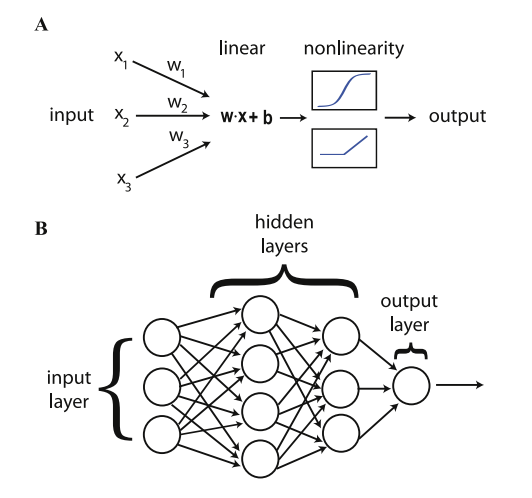
\includegraphics[width=\textwidth]{figures/basic_architecture.png}
        \end{column}
    \end{columns}
\end{frame}




\begin{frame}[fragile]{The FFNN}
\begin{lstlisting}[language=Python, frame=single, basicstyle=\fontsize{6}{6}\selectfont]
import torch
import torch.nn as nn
import torch.nn.functional as F

class Net(nn.Module):
    def __init__(self, N_dipoles: int, determine_area: bool = False, determine_amplitude: bool = False):
        super().__init__()
        self.determine_area = determine_area
        self.determine_amplitude = determine_amplitude
        self.fc1 = nn.Linear(231, 180)
        self.fc2 = nn.Linear(180, 120)
        self.fc3 = nn.Linear(120, 84)
        self.fc4 = nn.Linear(84, 16)
        if determine_amplitude:
            self.fc5 = nn.Linear(16, 5*N_dipoles)
        elif determine_area:
            self.fc5 = nn.Linear(16, 4*N_dipoles)
        else:
            self.fc5 = nn.Linear(16, 3*N_dipoles)

    def forward(self, x: torch.Tensor):
        x = F.relu(self.fc1(x))
        x = torch.tanh(self.fc2(x))
        x = torch.tanh(self.fc3(x))
        x = torch.tanh(self.fc4(x))
        x = self.fc5(x)

        return x
\end{lstlisting}
\end{frame}

\begin{frame}{Results (1) - Predicting coordinates}
  \begin{columns}
    \begin{column}{0.5\textwidth}
        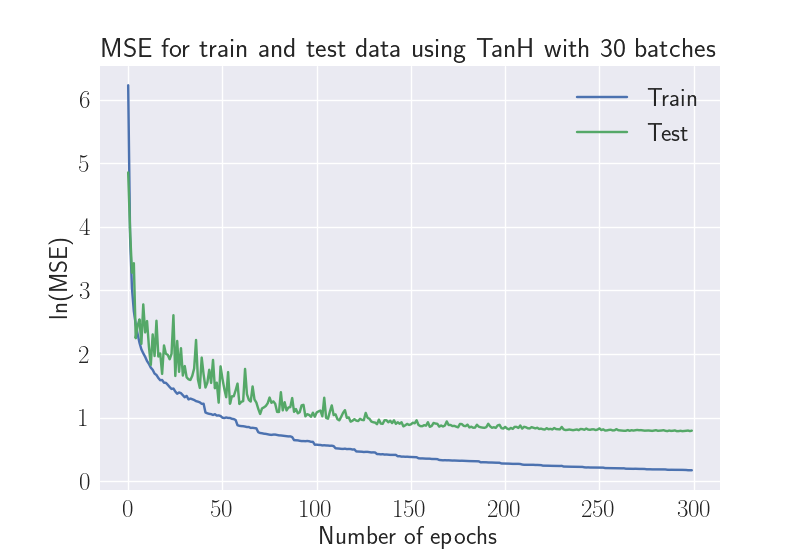
\includegraphics[width=\textwidth]{figures/MSE_simple_dipole_lr0.001_l1_penalty_300_50000_TanH_30_300_N_dipoles_1.png}
    \end{column}
    \begin{column}{0.5\textwidth}
        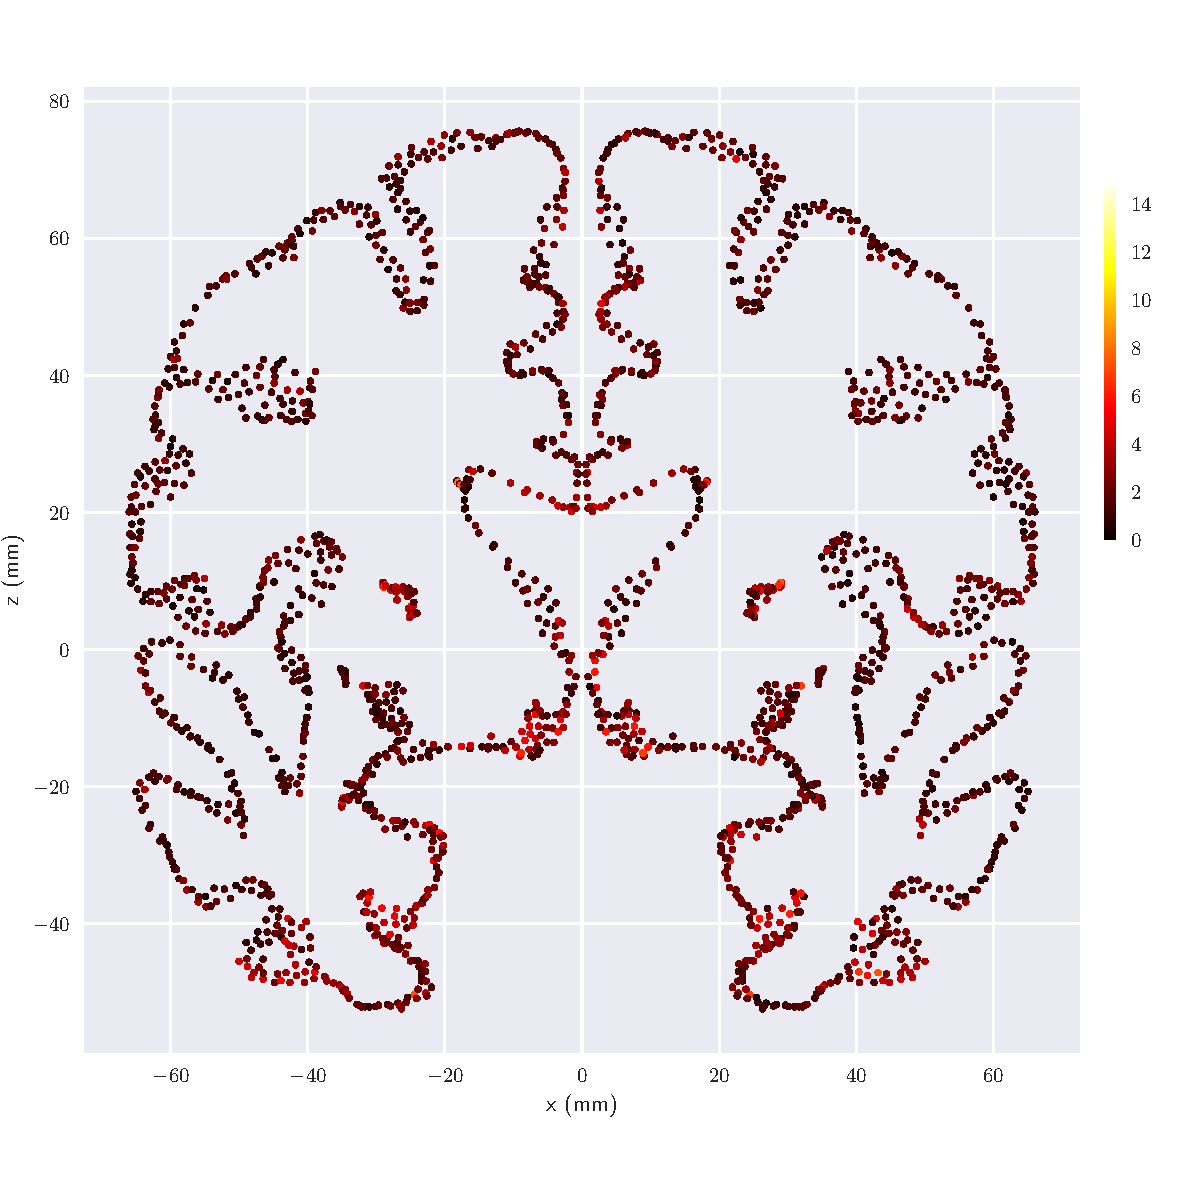
\includegraphics[width=0.7\textwidth]{figures/simple_dipole_error_position.pdf}
    \end{column}
  \end{columns}
\end{frame}

\begin{frame} \frametitle{Results (2)}
  \begin{table}
    \begin{tabular}{l|lll|}
      \cline{2-4}
      \rowcolor[HTML]{CBCEFB}
                                            & \multicolumn{3}{c|}{\cellcolor[HTML]{CBCEFB}\textbf{MAE for different models}}                                \\ \hline
      \rowcolor[HTML]{EFEFEF}
      \multicolumn{1}{|l|}{\textbf{Predictions}} & \cellcolor[HTML]{EFEFEF}\textbf{Location} & \cellcolor[HTML]{EFEFEF}\textbf{+ Amplitude} & \textbf{+ Radius} \\ \hline
      \multicolumn{1}{|l|}{x-coordinate [mm]} & 0.891                                     & 1.707                                       & 5.964             \\ \hline
      \multicolumn{1}{|l|}{y-coordinate [mm]} & 0.903                                     & 1.923                                       & 6.295             \\ \hline
      \multicolumn{1}{|l|}{z-coordinate [mm]} & 0.896                                     & 1.861                                       & 5.409             \\ \hline
      \multicolumn{1}{|l|}{Amplitude [nA]}   & -                                         & 0.619                                       & 339.9             \\ \hline
      \multicolumn{1}{|l|}{Radius [mm]}      & -                                         & -                                           & 2.094             \\ \hline
    \end{tabular}
  \end{table}
\end{frame}




\begin{frame}{Results (3) - Predicting coordinates for multiple dipole populations}
    \begin{columns}
        \begin{column}{0.5\textwidth}
            \begin{itemize}
              \item[$\bullet$] Typical example of overfitting
              \item[$\bullet$] NN are overly specialized to the specific training data and fail to generalize effectively
              \item[$\bullet$] Solution: Change architecture of NN (?)
            \end{itemize}
        \end{column}
        \begin{column}{0.5\textwidth}
            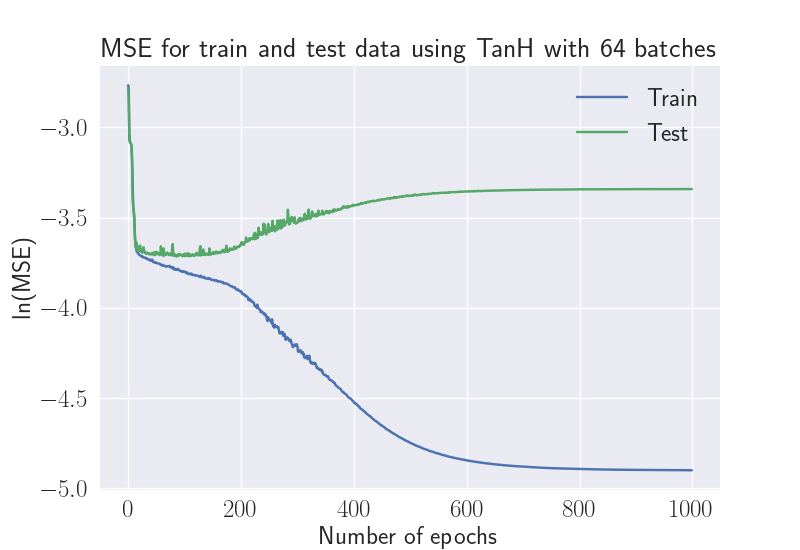
\includegraphics[width=\textwidth]{figures/MSE_10000_11may_MSE_area_w_amplitude_1000_SGD_lr1.5_wd0.1_mom0.35_bs64_TanH_64_1000_N_dipoles_2.png}
        \end{column}
    \end{columns}
\end{frame}

\begin{frame}{Summary}
    \begin{columns}
        \begin{column}{0.5\textwidth}
            \begin{itemize}
              \item[$\bullet$] Stronger fundation in managing, producing and analyzing large quantities of data
              \item[$\bullet$] Required proficiency in creative thinking and patience
              \item[$\bullet$] Further developed my programming skills
              \item[$\bullet$] Given the opportunity to developed and defeated bugs
            \end{itemize}
        \end{column}
        \begin{column}{0.5\textwidth}
            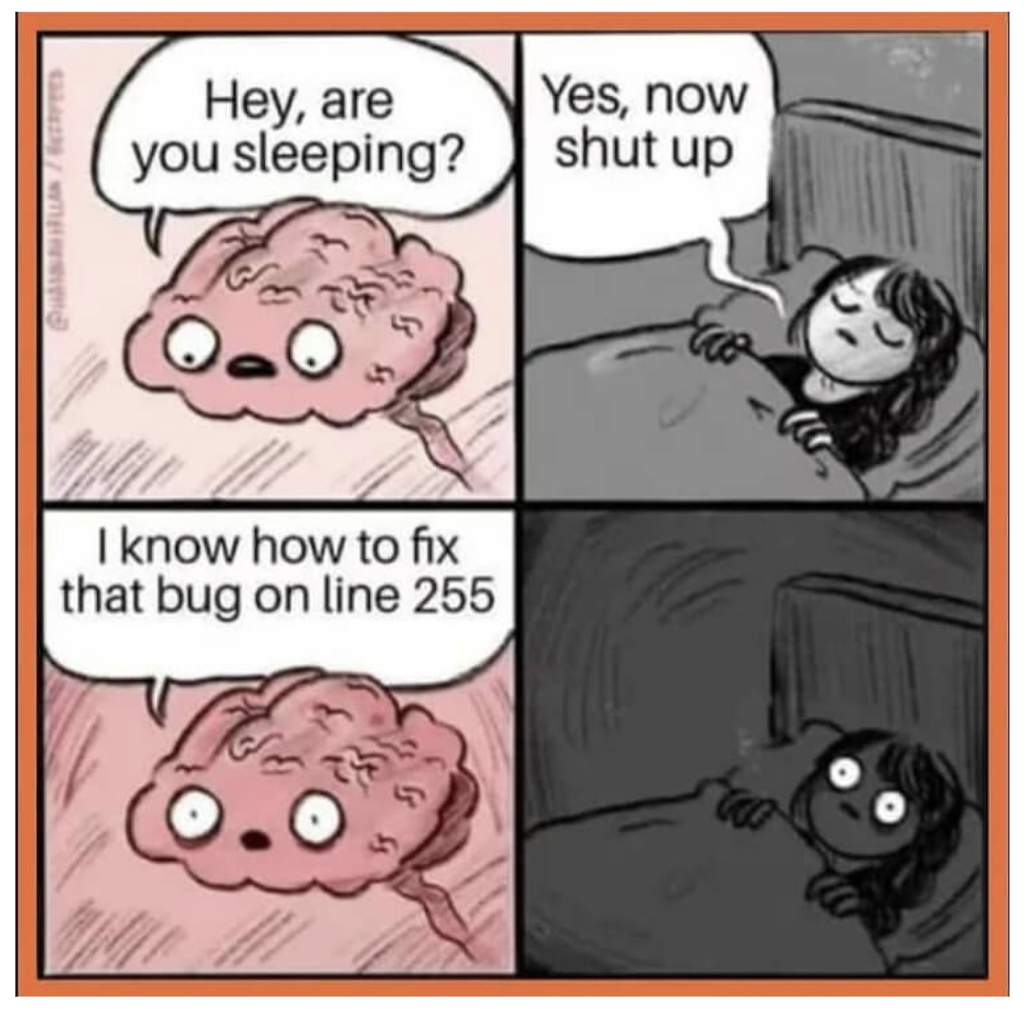
\includegraphics[width=0.7\textwidth]{figures/bugs.png}
        \end{column}
    \end{columns}
\end{frame}


\end{document}
